% Brett
\chapter{Experience with Kokkos}
\section{Performance}
%Comparing Kokkos to Cuda and OpenMP
%Doing this for sanity check
%How we did this (used same algorithm and ran both, timed)
%some graphical results
%analysis of the results and differences
%conclusion that they are very similar performing
A feature that many programmers consider when deciding what the best solution is
to solve their problem, is performance. Since Kokkos uses Cuda and OpenMP as a
backend we thought that it was important to do some testing to ensure that
Kokkos performs as well as these two solutions. If Kokkos's performance was
worse then Cuda's or OpenMP's then programmers would use these other solutions
instead. The good news for Kokkos is that in our testing it performs almost
identically to Cuda and OpenMP. We did not spend an extensive amount of time
confirming our results due to project priorities, but after a few pieces of supporting data we assumed that
the rest of the tests would give similar results because there is no information or evidence
that should give us reason to believe this trend will change. The rest of this
section will describe our strategy for testing performance of Kokkos versus Cuda
and Kokkos versus OpenMP, present graphs showing the differences observed, and
analyze the graphs.
\\
\\
The general method that was used to create performance data for Kokkos, Cuda,
and OpenMP was to write algorithmically equivalent code for all three, make sure
that the layout of the data is the same, then time the runtime of each (one
after another). This process is pretty simple, but there is always noise in
timing. That is why we repeated the same exact calculation five times and 
then use the average time. A couple things that should be noted are we are
unsure how Kokkos does a reduction in the team\_reduce() function, meaning we
could not write a Cuda reduction that we knew was algorithm equivalent, and we
can not be sure that the compilers do the same optimizations. Although
we could have asked Dr. Carter Edwards (our liaison and one of the creators of 
Kokkos), the project's priorities had changed and it was decided to not pursue
this further. Regarding the second note, we tried to manually do some code
optimizations that compilers can handle in order to make sure the amount of work
each algorithm was the same (which is expected). Of course if one compiler has
more advanced optimization techniques that is a benefit that should not be
overlooked, but the goal of this testing was not to test performance against
ease of coding, but rather the overall performance differences of Kokkos to 
Cuda and Kokkos to OpenMP. \\
\\
Now we will look at some of the performance differences and similarities of
Kokkos, Cuda, and OpenMP. Here is a graph that shows the raw times of Kokkos
Cuda, Cuda, Kokkos OpenMP, and OpenMP for ContractDataDataScalar: \\
\begin{figure}[!ht]
{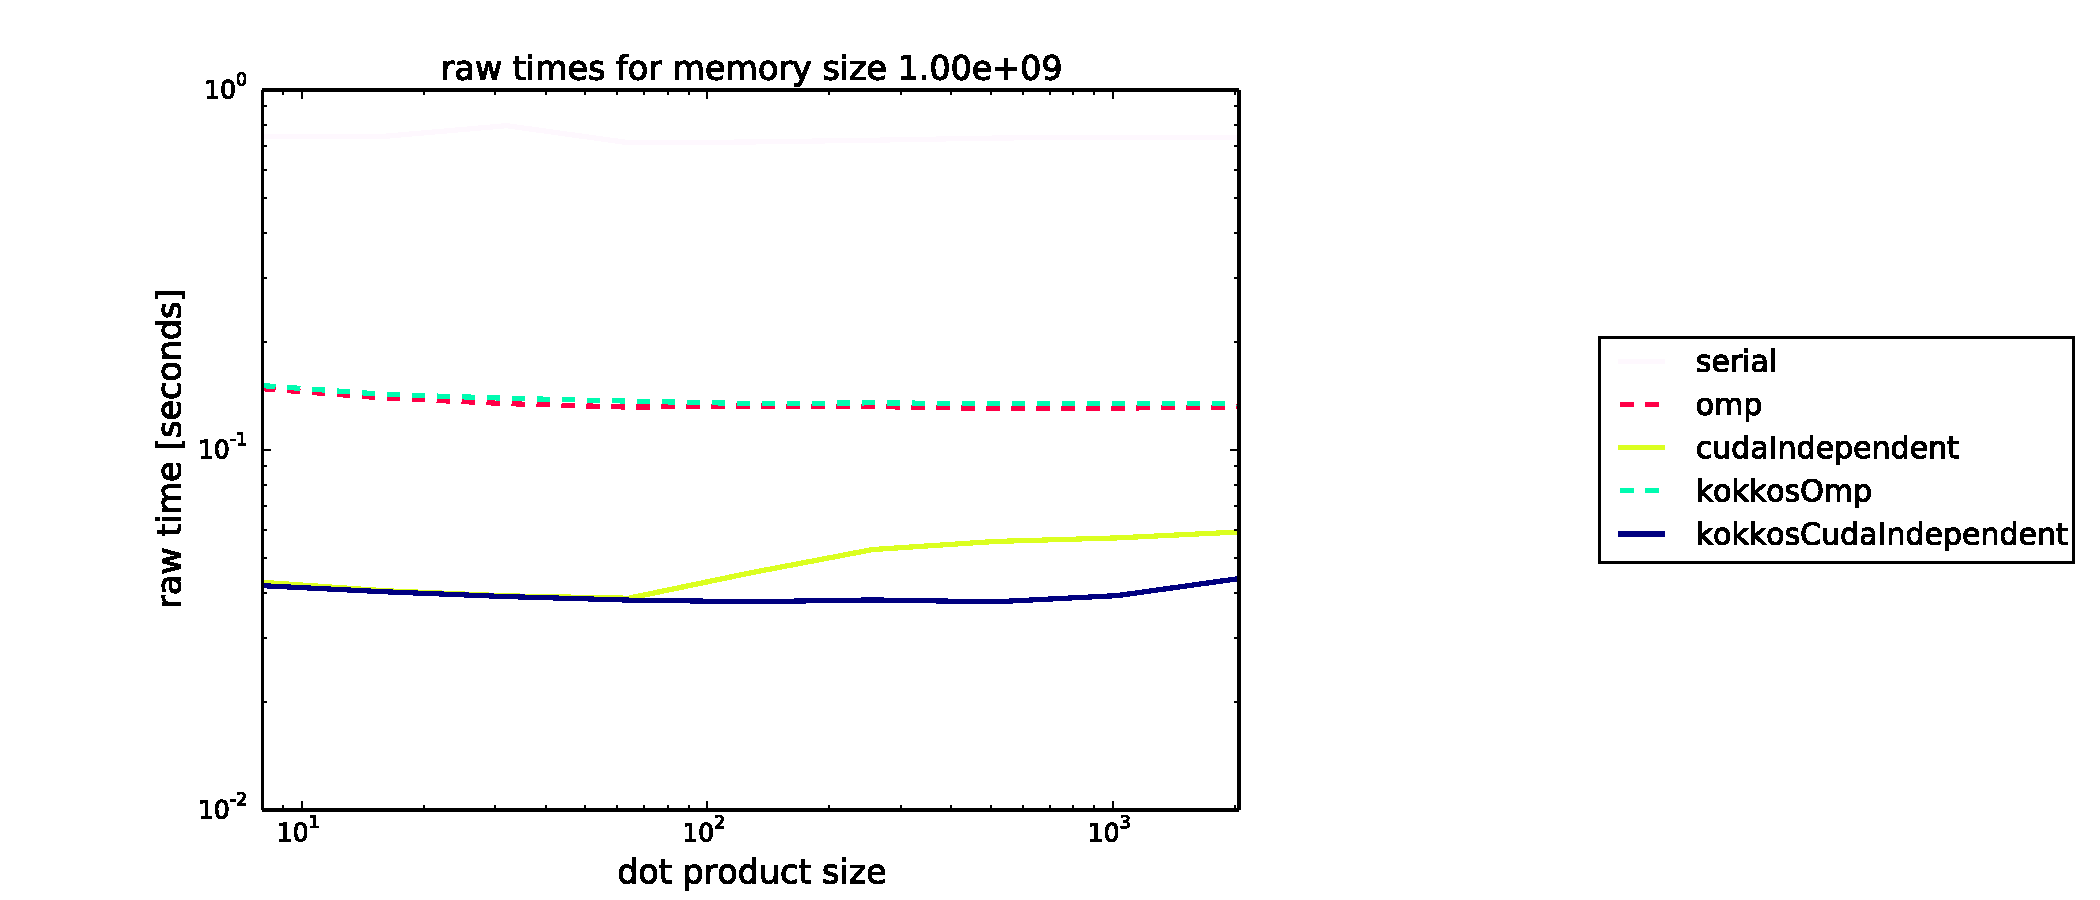
\includegraphics[scale=.4]{CDDS_RawTimes_2d_largestSize_Comparison.pdf}}
\caption[ContractDataDataScalar Kokkos performance comparison]{This graph plots the performance of Kokkos Cuda, Cuda, Kokkos OpenMP,
and OpenMP for ContractDataDataScalar with a memory size of 1 GB. 
The y-axis is time in
seconds, so closer to 0 is better. The x-axis plots different contraction sizes
in order to compare multiple points.}
\label{fig:ContractDataDataScalar Kokkos performance comparison}
\end{figure} \\
Notice how in this graph Kokkos OpenMP and OpenMP are almost perfectly
overlapping with Kokkos OpenMP. We are not quite sure why they are not perfectly
overlapping, but it appears that it is not random noise because it is pretty
consistent in this graph. However, the difference is so small it seems
insignificant. \\
\\
KokkosCuda versus Cuda, on the other hand, has some big differences. They are
identical for the smaller problems but diverge a significant amount for bigger
problems. One of the theories that we have as to why this trend exists is that
Kokkos may be launching a different amount of blocks than the number of blocks Cuda launches.
We believe the reason this doesn't effect the smaller problem sizes is because
the number of blocks that needs to be launched is smaller than the bigger problem sizes, so
the upper limit of number of blocks launched is not reached, but clearly is in the bigger problem sizes. \\
\\
Now here is a graph for ContractFieldFieldScalar that includes the slicing technique (which uses shared memory)
for both Kokkos Cuda and Cuda and it includes the normal flat parallel algorithm for Kokkos Cuda and Cuda. \\
\begin{figure}[!ht]
{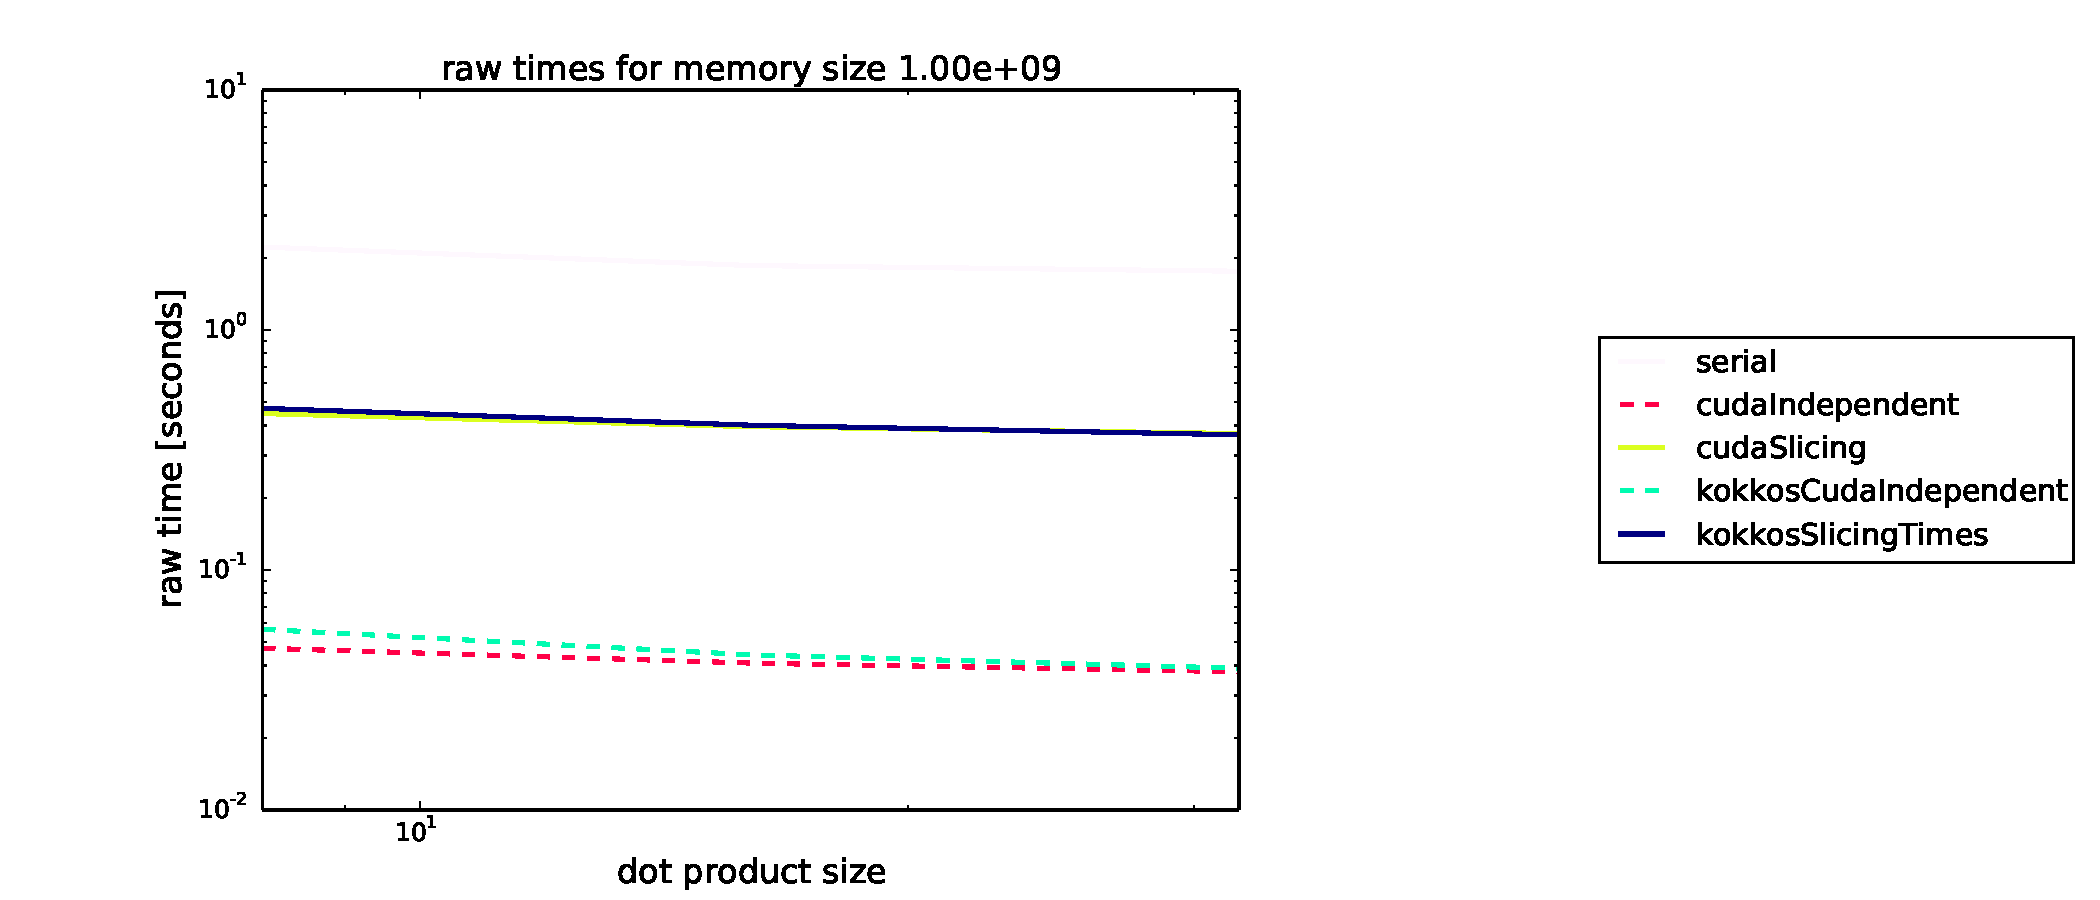
\includegraphics[scale=.4]{CFFS_RawTimes_2d_largest_Comparison.pdf}}
\caption[ContractFieldFieldScalar Kokkos performance comparison]{This graph shows performance differences (or similarities in our case)
of the nested parallelism approach slicing.}
\label{fig:cffscomparison}
\end{figure} \\
In this graph it is clear that the Cuda slicing performance is almost identical
to the Kokkos slicing performance. This is important to show that both Kokkos's
and Cuda's use of shared memory results in the same performance. \\
\\
Overall, after seeing a handful of graphs that show Kokkos performs almost
identically to Cuda and to OpenMP, we accepted that Kokkos is not adding any
unneeded overhead. As stated before, there may be slight differences due to
compiler optimizations, but Kokkos seems to perform identically to the other
multithreading solutions.

\section{Snippets}
%Amount of work the programmer has to do is important
%control and complexity of code is important
%Much more complex than OpenMP, but follows a different paradigm
%Very similar to Cuda, except kernel is a functor
%Overall a pretty easy language, some magic values but pretty good
Another major factor that plays into whether or not a programmer uses a certain
language, feature, library, etcetera, is code complexity and ease of coding.
Although this can be subjective, there are a couple differences between the
language we would like to point out, especially regarding amount of code
required compared to Cuda or OpenMP (although comparing to OpenMP may be unfair)
and intuitiveness of the code (or readability). \\
\\
Regarding the amount of code required, comparing Kokkos to OpenMP does not seem
fair. Comparing OpenMP to almost anything seems unfair, because OpenMP requires
very little code and most of the work is done for you. Although OpenMP only
works on the CPU which is why it does not require the extra code that Kokkos
requires. In general, OpenMP cannot be compared to Kokkos. If the programmer
knows the code only needs to be multithreaded on the CPU and will never need
more threads then we would strongly advise them to use OpenMP because it is very
simple. However, that is not the niche that Kokkos is trying to fill. \\
\\
Kokkos compared to Cuda however, requires similar amounts of code. 
Throughout the code comparison of Cuda and Kokkos we will show
code snippets and point out the differences and similarities directly. We will
start by showing the data setup, because the data needs to get onto the GPU
somehow, then we will move to compare and contrast the Cuda kernel and the Kokkos
functor. \\
\\
Here is code that shows the setup of the data on the GPU for Cuda: \\
\begin{figure}[!htb]
	\begin{lstlisting}
float * dev_leftDataArray;
checkCudaError(cudaMalloc((void **) &dev_leftDataArray, 
	numContractions * numLeftFields * numPoints * 
	sizeof(float)));
	
checkCudaError(cudaMemcpy(dev_leftDataArray, &leftDataArray[0], 
	numContractions * numLeftFields * numPoints * sizeof(float), 
	cudaMemcpyHostToDevice));
	\end{lstlisting}
\caption{Code from Cuda \texttt{ContractFieldFieldScalar}
\label{lst:ContractFieldFieldScalar Cuda Data Setup}}
\end{figure}
\\
There are essentially three steps in the process: declaring a pointer to the
data on the CPU, creating an array with the correct size on the GPU, then
copying the data over to the GPU from wherever the data is currently kept on the
CPU. This process is pretty simple and self-explanatory. Now let us compare that
to Kokkos: \\
\begin{figure}[!htb]
	\begin{lstlisting}
typedef Kokkos::Cuda	DeviceType;
typedef Kokkos::View<float***, Kokkos::LayoutRight, DeviceType>
	ContractionData;
typedef typename ContractionData::HostMirror
	ContractionData_Host;

ContractionData dev_ContractData_Left("left_data",
	numContractions,
	numLeftFields,
	numPoints);

ContractionData_Host contractionData_Left = 
	Kokkos::create_mirror_view(dev_ContractData_Left);

for (int cell = 0; cell < numContractions; ++cell) {
	for (int lbf = 0; lbf < numLeftFields; ++lbf) {
		for (int qp = 0; qp < numLeftFields; ++qp) {
			contractionData_Left(cell, lbf, qp) = 
				contractionDataLeft[cell*numLeftFields*
				numPoints + lbf*numLeftFields + qp];
		}
	}
}
	\end{lstlisting}
\caption{Code from Kokkos Cuda \texttt{ContractFieldFieldScalar}
\label{lst:ContractFieldFieldScalar Kokkos Cuda Data Setup}}
\end{figure}
\\
The Kokkos code first defines and creates the device and host views. One of the major differences compared to Cuda is that Kokkos uses its own data structure, a View, instead of an array. This is why we need to use typedefs to define the Views, but the extra work (which honestly is not much of a hassle) allows the programmer much more control over the data. The control also comes at the cost of having to use for loops to copy the data into the host view instead of being able to do a Memcpy. However, this is all initial work that needs to be done once, while the benefit of being able to change the layout of the data by changing the Kokkos::LayoutRight to Kokkos::LayoutLeft is very useful, especially since this allows the programmer to optimize data layout for both the CPU and GPU. Overall, Kokkos' and Cuda's data setup have different philosophies, which makes sense because Kokkos needs to be easily optimized for both the CPU and GPU while Cuda only runs on the GPU. \\
\\
Looking at the "guts" of the programs, Cuda has a kernel that is launched where all the computation is, while Kokkos uses a functor, almost identical to Intel's Thread Building Blocks threading paradigm. However, for programs doing the same calculation, the parenthesis operator function in Kokkos' functor is almost an exact replica of the code in Cuda's kernel. Here is the code for a Cuda kernel for ContractFieldFieldScalar: \\
\begin{figure}[htb]
	\begin{lstlisting}
__global__ void
cudaContractFieldFieldScalar_Flat_kernel(int numContractions,
	int numLeftFields,
	int numRightFields,
	int numPoints,
	float * __restrict__ dev_contractData_Left,
	float * __restrict__ dev_contractData_Right,
	float * dev_contractResults) {
	int contractionIndex = blockId.x * blockDim.x + threadIdx.x;
	while (contractionIndex < numContractions) {
		int myID = contractionIndex;
		int myCell = myID / (numLeftFields * numRightFields);
		int matrixIndex = myID % (numLeftFields * numRightFields);
		int matrixRow = matrixIndex / numRightFields;
		int matrixCol = matrixIndex % numRightFields;
		
		// Calculate now to save computation
		int lCell = myMatrix * numLeftFields * numPoints;
		int rCell = myMatrix * numRightFields * numPoints;
		int resultCell = myMatrix * numLeftFields * numRightFields;
		
		float temp = 0;
		for (int qp =0; qp < contractionSize; qp++) {
			temp += dev_contractData_Left[lCell + 
				qp*numLeftFields + matrixRow] *
				dev_contractData_Right[rCell + 
				qp*numRightFields + matrixCol];
		}

		dev_contractResults[resultCell + 
			matrixRow * numRightFields + matrixCol] = temp;
		
		contractionIndex += blockDim.x * gridDim.x;
	}
}
	
	\end{lstlisting}
\caption{Code from Cuda \texttt{ContractFieldFieldScalar}
\label{lst:ContractFieldFieldScalar Cuda kernel}}
\end{figure}
\\
\begin{figure}[htb]
	\begin{lstlisting}
KOKKOS_INLINE_FUNCTION
void operator() (const unsigned int elementIndex) const {
	int myID = elementIndex;
	int myCell = myID / (_numLeftFields * _numRightFields);
	int matrixIndex = myID % (_numLeftFields * _numRightFields);
	int matrixRow = matrixIndex / _numRightFields;
	int matrixCol = matrixIndex % _numRightFields;

	float temp = 0;
	for (int qp = 0; qp < _numPoints; qp++) {
		temp += _leftFields(myCell, qp, matrixRow) *
			_rightFields(myCell, qp, matrixCol);
	}
	_outputFields(myCell, matrixRow, matrixCol) = temp;
}
	\end{lstlisting}
\caption{Code from Kokkos Cuda \texttt{ContractFieldFieldScalar}
\label{lst:ContractFieldFieldScalar Kokkos Cuda functor}}
\end{figure}
\\
Kokkos operator () less cluttered than Cuda. Better indexing into data. Having functor save important data vs passing as arguments is nice. 


\section{Personal Experience and Thoughts}
% Positive experience
% We don't know how to install kokkos and took a while to get things to compile
% Magic word hassles 
% Following examples we can figure out what to do by copying syntax
% No documentation when we wanted to figure out what exactly was happening
% 
A task of the project was to document our experiences and thoughts about Kokkos, including any issues that we have run into. Using new tools and learning new syntax always has its tough periods, and getting used to Kokkos definitely had some periods where we had no idea why a program was not compile or giving an incorrect answer (especially in the beginning), but after the initial learning curve everything seemed to flow pretty well and make sense. \\
\\
Our team has never actually been responsible for installing Kokkos on our machine, instead our liaison, Dr. Carter Edwards, did that for us, so we are unable to talk about the difficulties of downloading and installing the Kokkos library on our machine, but we did have lots of trouble trying to compile and linking against Kokkos originally. This was due to the fact that the same flags need to be used when installing and compiling and linking against Kokkos. However, since we did not install Kokkos ourselves and the documentation showing how to compile and link against Kokkos used different flags than what were used during our installation, we struggled for a while. Already this shows how Kokkos' documentation is not as developed as one would like, which we will bring up later, but it is understandable since Kokkos is new. \\
\\
Another obstacle that slowed us down when first using, is Kokkos' use of magic words. For example, Kokkos requires the programmer to typedef Kokkos::Cuda or Kokkos::OpenMP to device\_type, and it must be device\_type, not some other name. Although the programmer can easily fix this, if the programmer is unaware of this requirement it can cause a lot of hassle for a while. Every team member ran into this at one time or another, but after a while we got used to it. When following examples we learned to use the same names for the typedefs to make sure that we did not run into another bug with the same nature. Once again documentation would have helped in this situation, but there is not much documentation all we have are examples. On the bright side however, since we were able to write all of our programs by simply following a few examples we were able to see some of Kokkos' intuitiveness. Overall we really enjoy Kokkos' philosophy and structure, which as mentioned before, is almost identical to Intel's Thread Building Blocks (TBB). If you are familiar with TBB then learning Kokkos is almost as simple as learning the syntax because they are in the same paradigm. 
